% Chapter 3

\chapter{前端设计}

网站主要采用W3 CSS样式进行修饰,主要使用灰白黑三种颜色,风格较为简约、清爽。整个网站系统包含欢迎界面、主界面、登录界面、注册界面、文件详情页面等共计12个子页面。

\section{欢迎界面}

欢迎界面是用户打开本系统所看到的第一个页面,即本系统的门户。

欢迎界面的上方是本系统的名称——SigDict。同时这部分也是本系统公用的,这部分将重复出现于后续的所有界面中。

欢迎界面的左侧是一片小短文,其中简要解释了本项目的起源、特性以及简要用途。

欢迎界面的右侧有引导用户登录和注册的按钮,用户点击后会分别打开两个新的页面,完成登录或者注册的操作。

\begin{figure}[!htb]
	\centering
	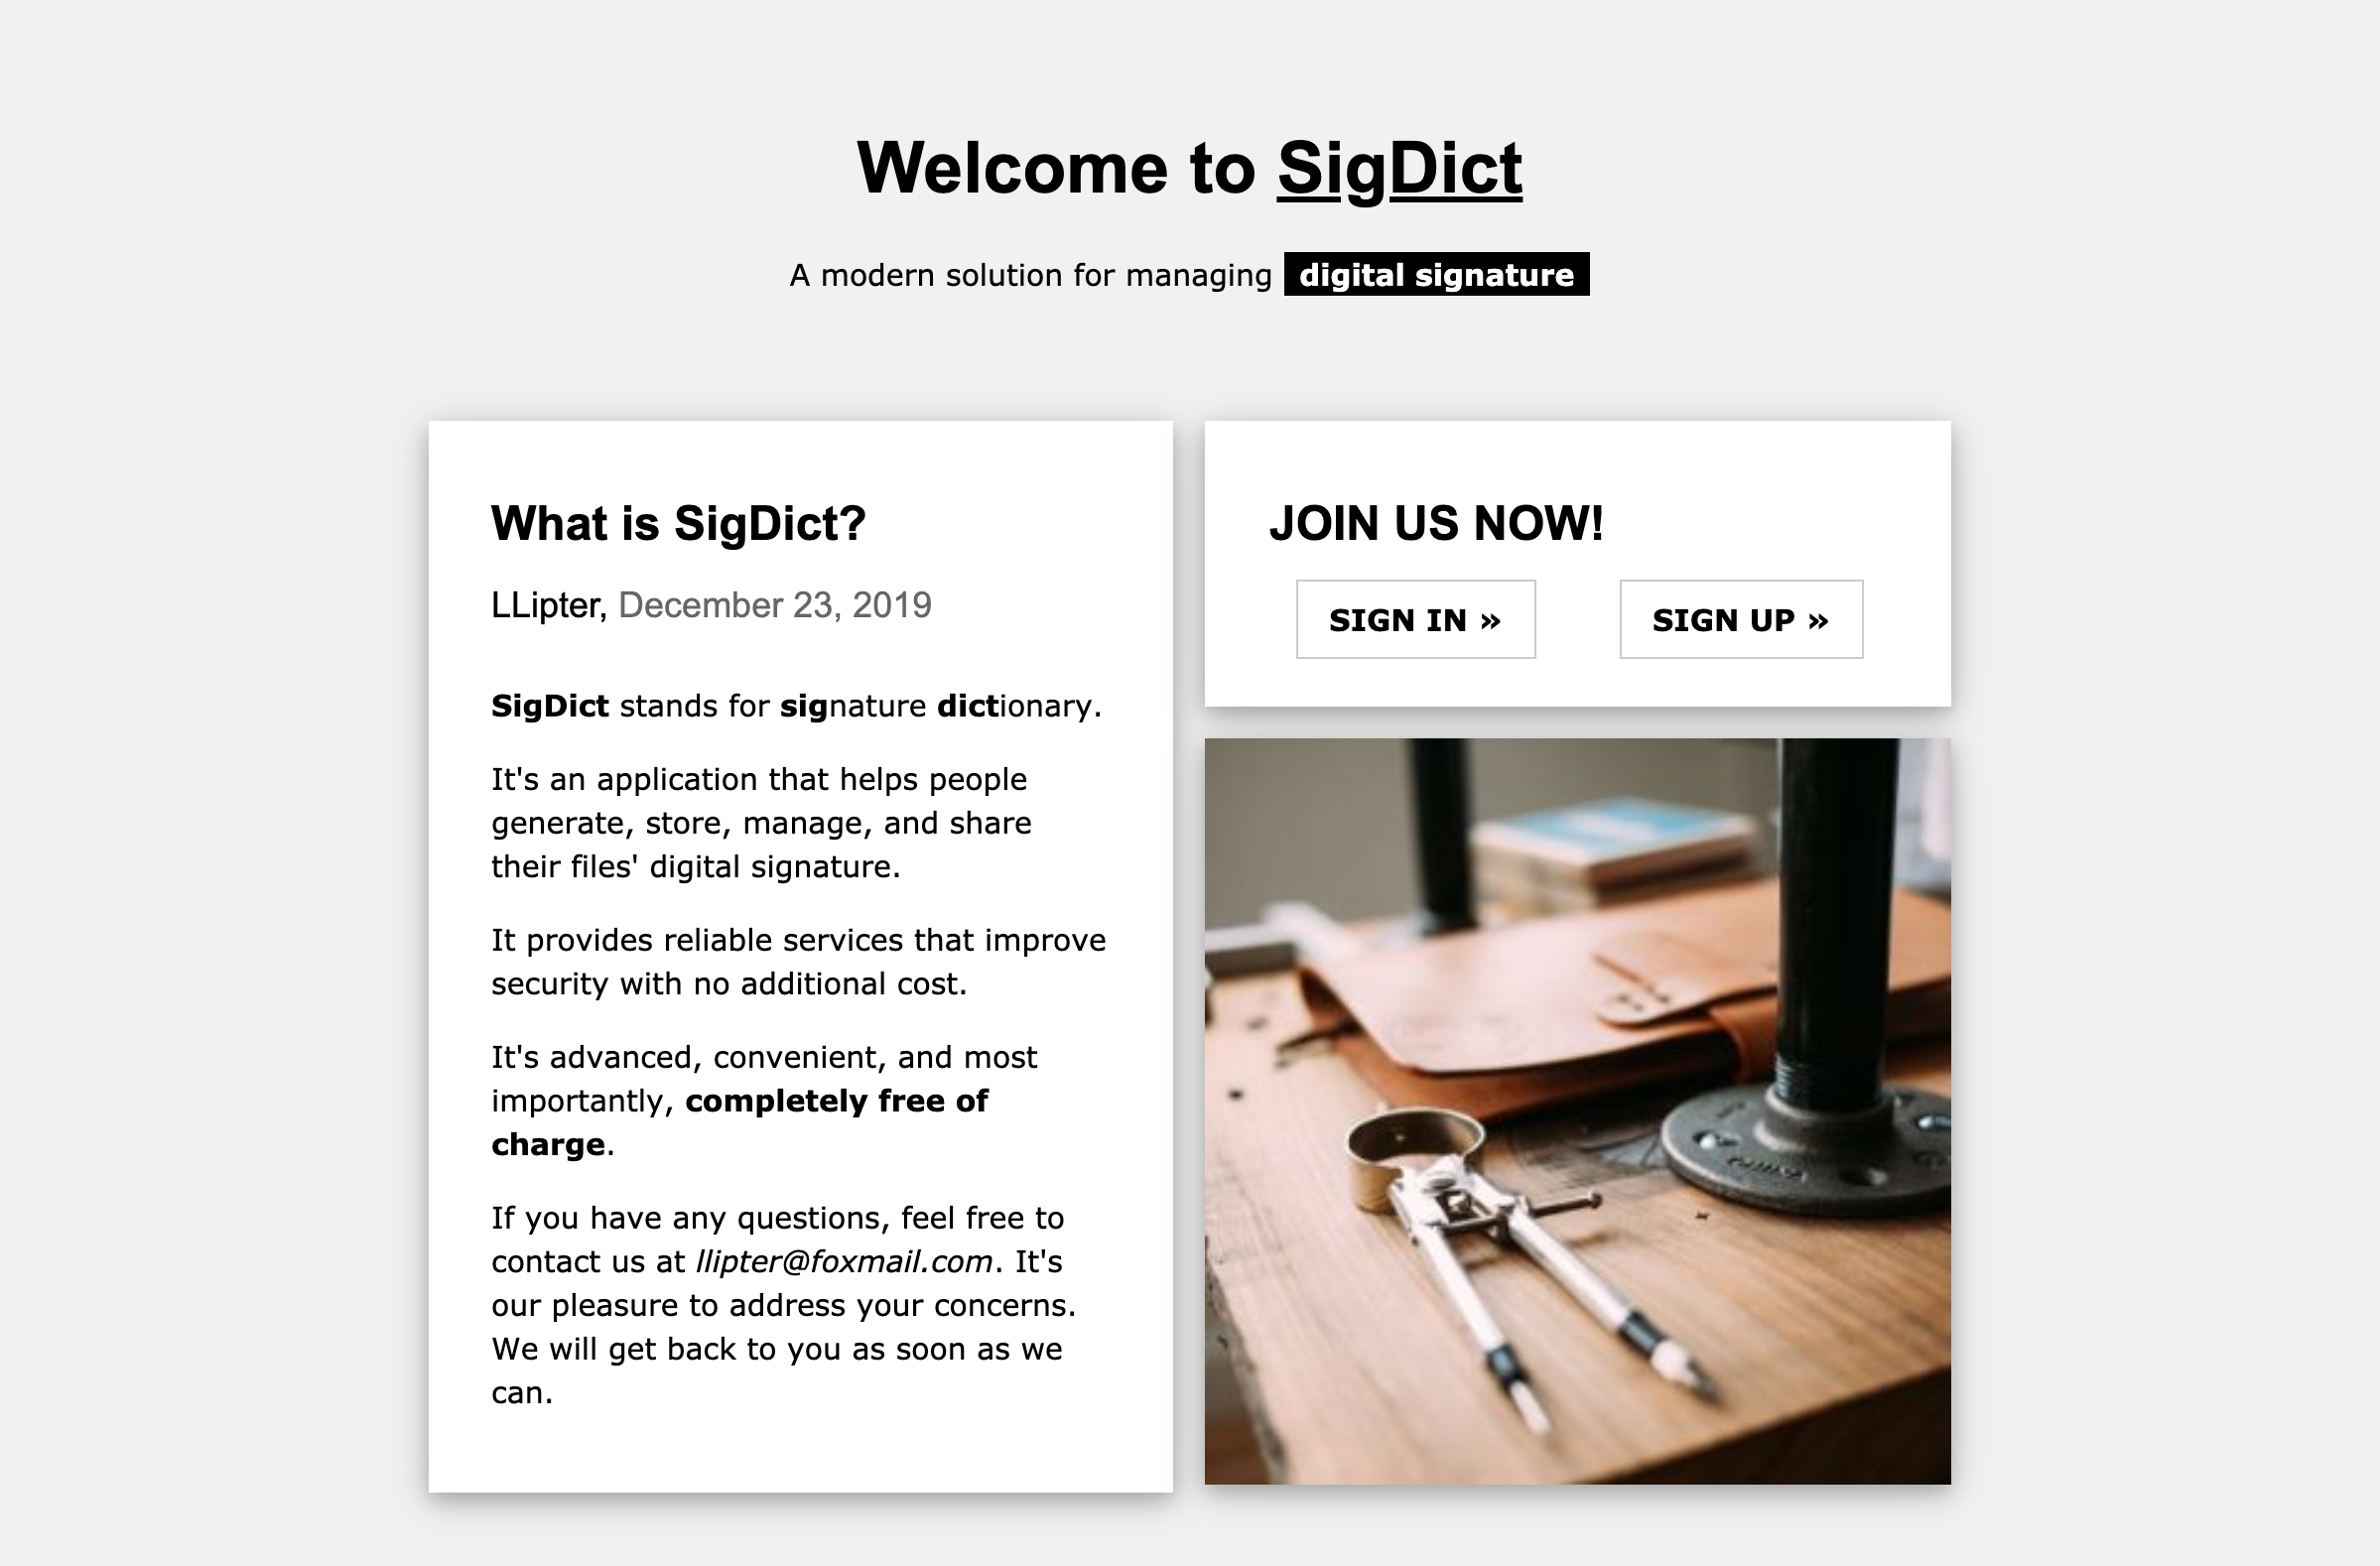
\includegraphics[width=0.8\textwidth]
	{figures/index.png}\\
	\caption{欢迎界面}
	\label{fig:index}
\end{figure}

\section{登录和注册界面}

在登录界面中,用户需要输入用户名和密码,在校验正确后即可成功登录。而如果用户忘记密码可以点击“FORGET PASSWORD”,通过验证过的邮箱重置密码。

在注册界面中,用户需要输入用户名、电子邮箱地址、密码、第二次密码确认这四项信息。在上述四项信息全部校验正确后注册成功,并跳转到主界面。校验规则将在小节\ref{sec:registerV}中具体介绍。

\begin{figure}[!htb]
	\begin{minipage}[t]{0.5\textwidth}
		\centering
		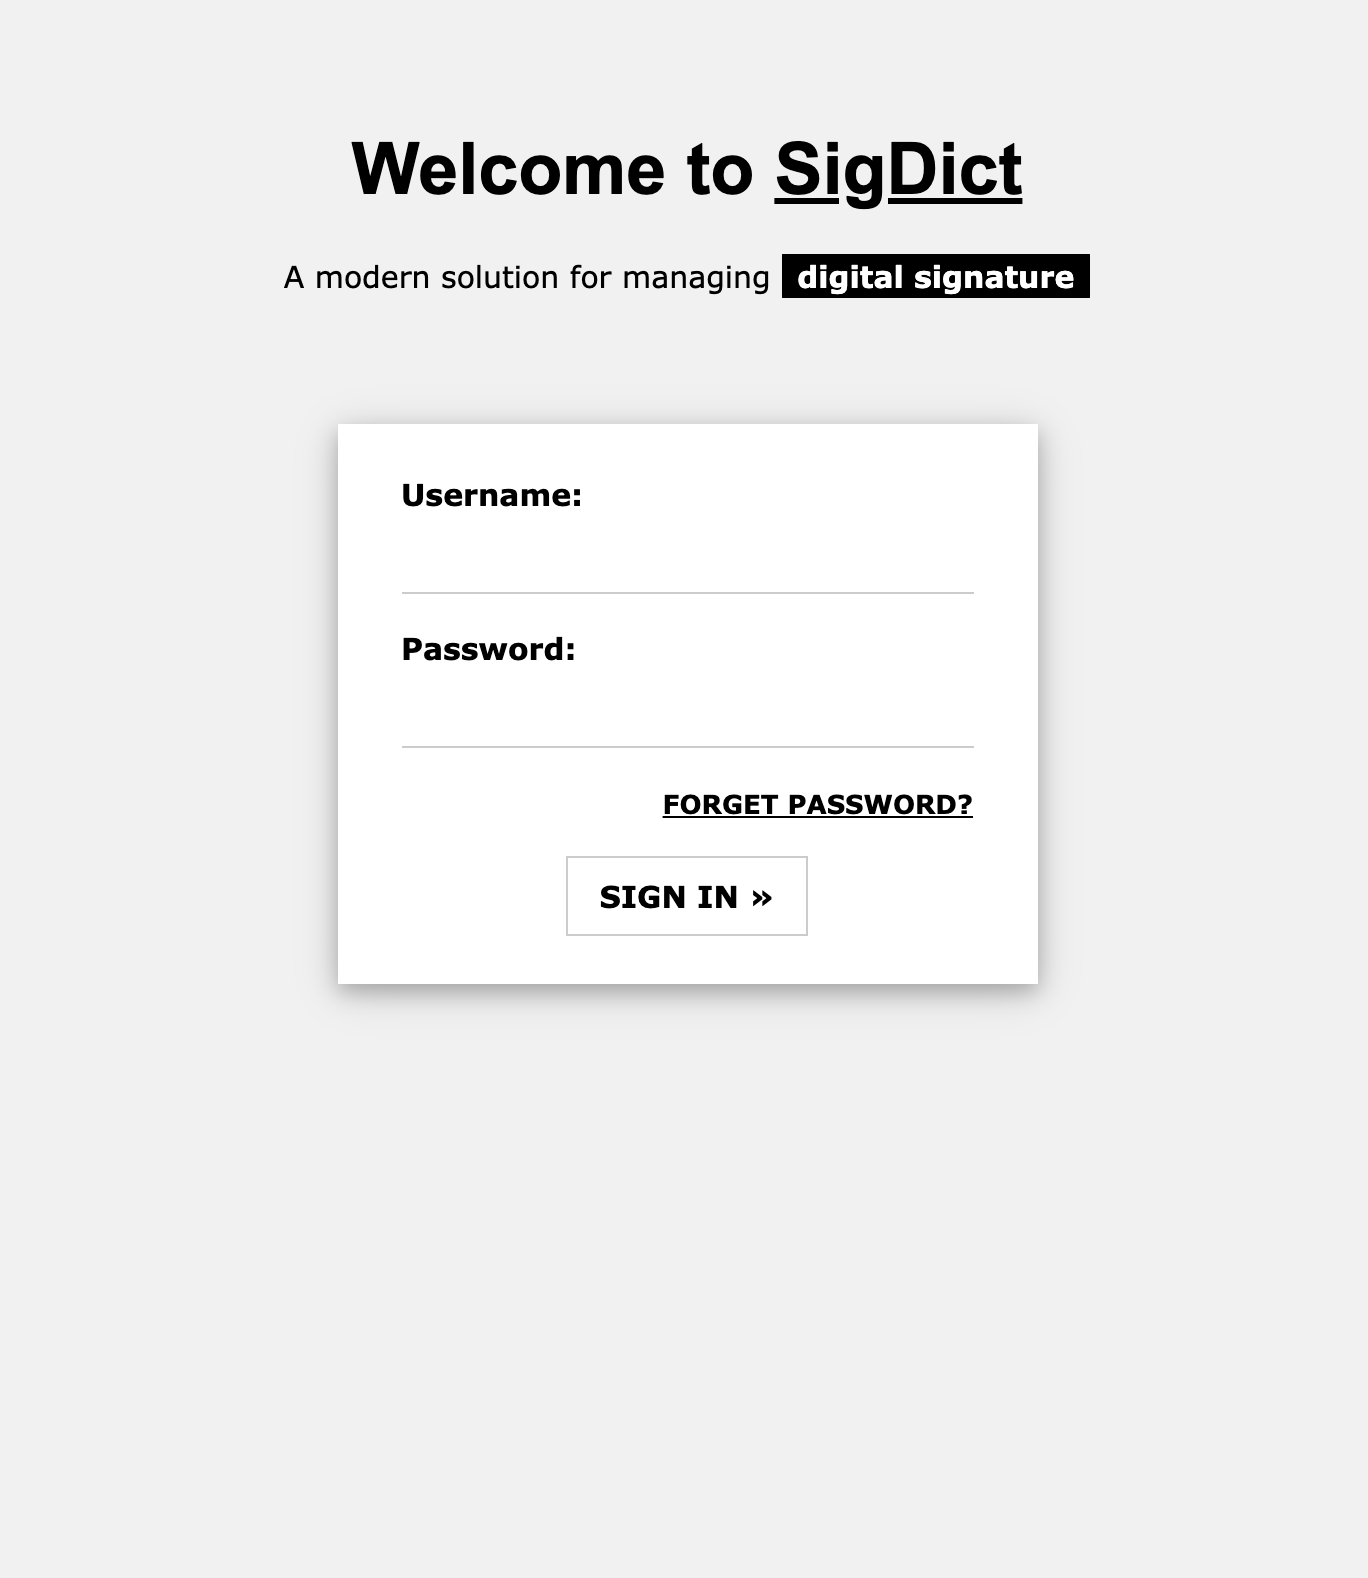
\includegraphics[width=1\textwidth]
		{figures/login.png}\\
		\caption{登录界面}
		\label{fig:login}
	\end{minipage}
	\qquad
	\begin{minipage}[t]{0.5\textwidth}
		\centering
		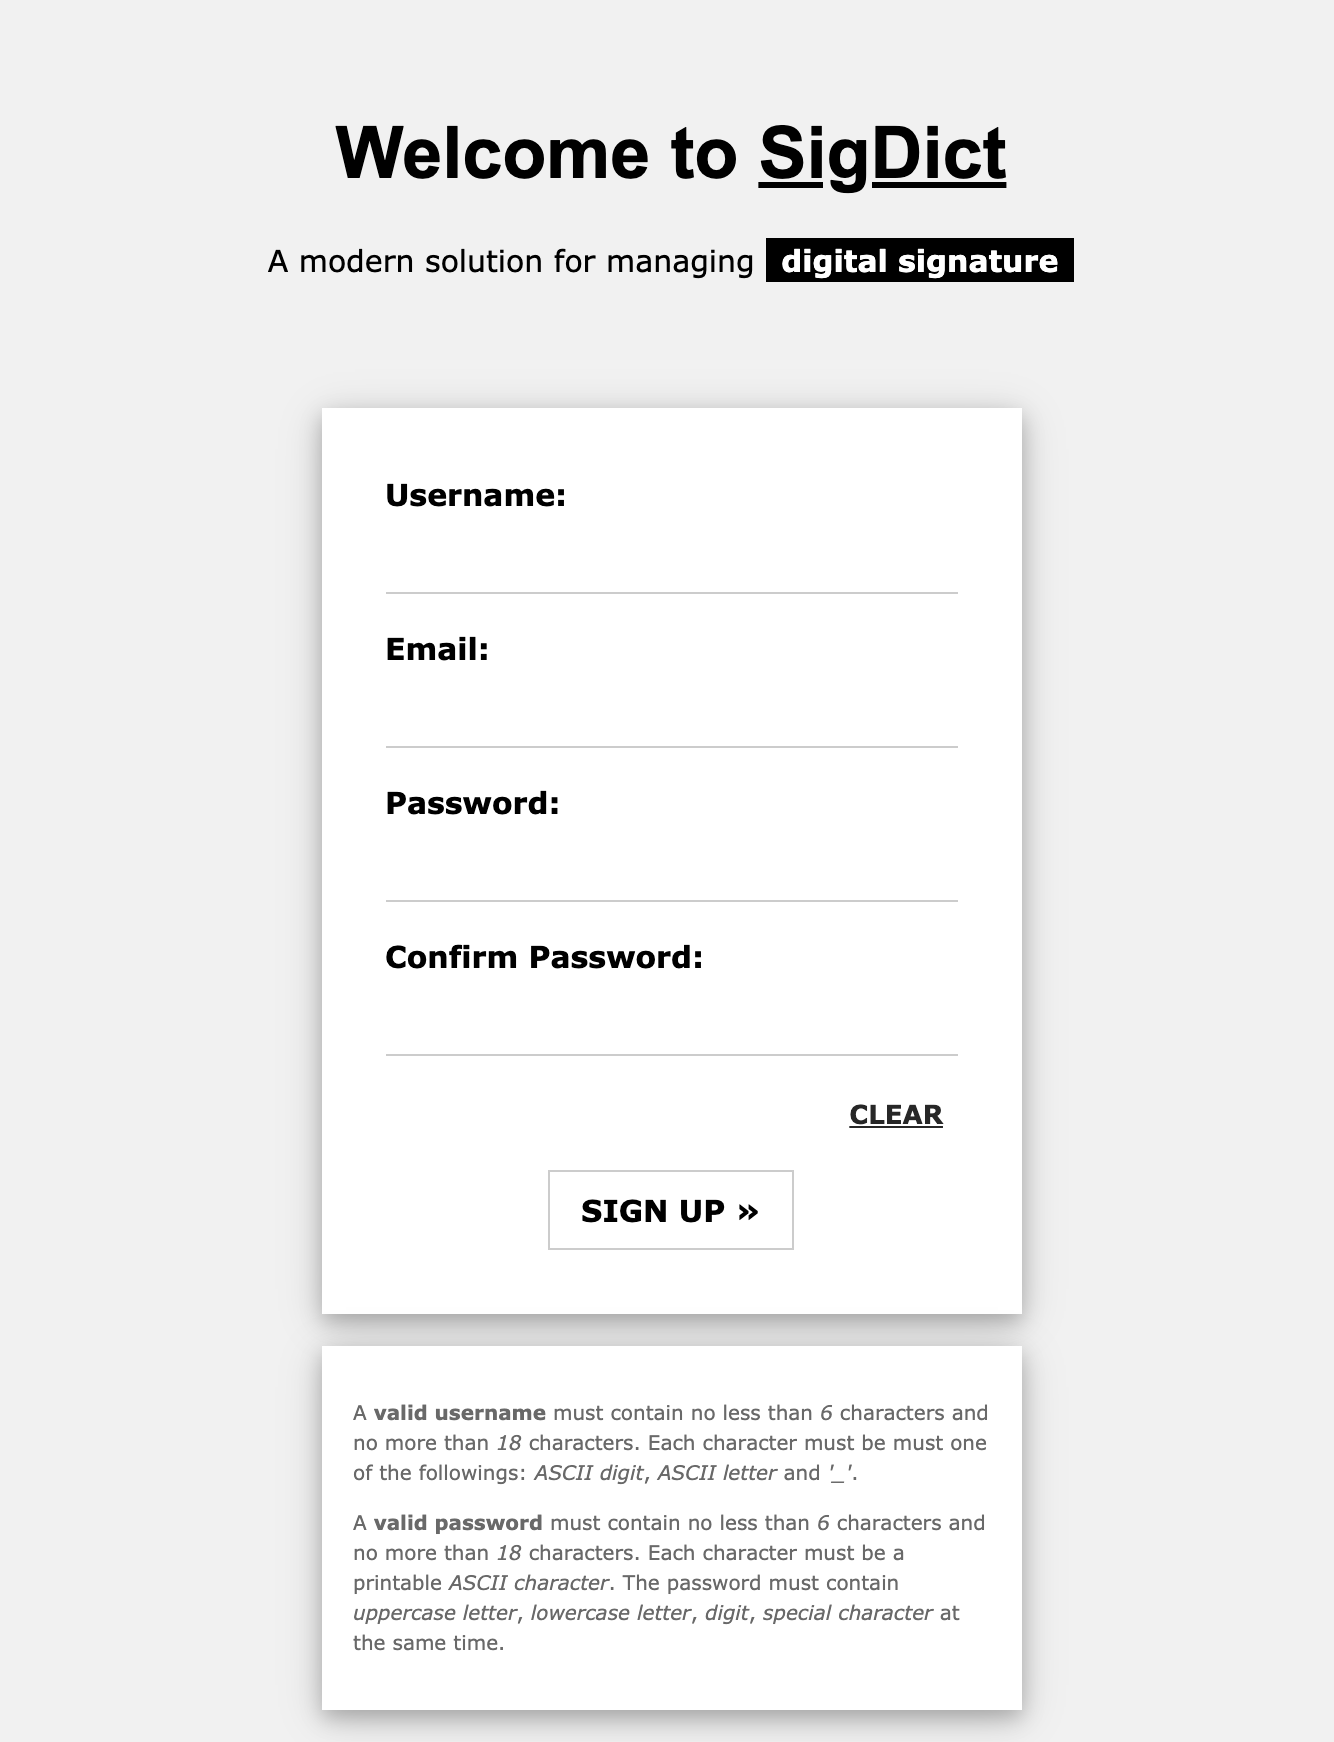
\includegraphics[width=1\textwidth]
		{figures/register.png}\\
		\caption{注册界面}
		\label{fig:register}
	\end{minipage}
\end{figure}
